%ChapterIII.tex
\section{随机过程}
    随机过程就像一个每一个面画着不同波形的骰子\footnote{\url{https://www.bilibili.com/video/BV11x411G79C?p=17}中杨鸿文老师的比喻。}。
    每次掷骰子获得的是一个在时域上的波形,如果单就个时间点看来,获得的就算是一个随机样本了\footnote{具体定义还是看书上27页叭}。

    随机过程的两个含义:
    \vspace{-2ex}
    \paragraph{}某一个确定的时刻,随机过程表现为一个随机变量。
    \vspace{-2ex}
    \paragraph{}随机过程$X(t)$的一个具体取值形成一个样本函数,用$x(t)$表示。
    \vspace{1ex}

    与书中相似的,使用大写字母表示随机变量或随机过程,小写字母表示具体的实现(或者说样本)。

\subsection{随机过程的统计特性}
    随机过程的统计性质可由其\emph{分布函数}和\emph{概率密度}函数描述

    \subsubsection{单个随机过程的数字特征}

    随机过程$X(t)$的一维\emph{分布函数}:
    \begin{equation}
        F_1(x_1,t_2)=\text{Pr}\{X(t_1)\leq x_1\}
    \end{equation}

    随机过程$X(t)$的一维\emph{概率密度函数}:
    \begin{equation}
        \frac{\partial F_1(x_1,t_1)}{\partial x_1}=p_1(x_1,t_1)
    \end{equation}

    随机过程$X(t)$的$n$维\emph{分布函数}:
    \begin{equation}
        \begin{split}
            &F_n(x_1,x_2,\cdots,x_n;t_1,t_2,\cdots,t_n)\\
            &\phantom{F_n}=\text{Pr}\{X(t_1)\leq x_1,X(t_2)\leq x_2,\cdots ,X(t_n)\leq x_n\}
        \end{split}
    \end{equation}

    随机过程$X(t)$的$n$维\emph{概率密度函数}:
    \begin{equation}
        \frac{\partial^n F_n(x_1,x_2,\cdots,x_n;t_1,t_2,\cdots,t_n)}{\partial x_1\partial x_2\cdots\partial x_n}=p_n(x_1,x_2,\cdots,x_n;t_1,t_2,\cdots,t_n)
    \end{equation}

    使用算子$\mathscr{E}$或$E$代表\emph{统计平均},统计平均是对某一个确定时刻$t$时所有可能的样本的期望值,
    与之相对的$\overline{(\cdot)}$则是某个算式(可能是关于时间的函数)在整个时域上的平均值。

    随机过程$X(t)$的\emph{数学期望}:
    \begin{equation}
        \mathscr{E}[X(t)]=\int_{-\infty}^{\infty}xp_1(x,t)\dif x=m_X(t)
    \end{equation}
    显而易见的,任意个随机过程总可以看作是一个\emph{零均值}的随机过程和一个确定函数的和
    \begin{equation}
        X(t)=\widetilde{X}(t)+m_X(t)
    \end{equation}

    同样的,随机过程$X(t)$的\emph{方差}:
    \begin{equation}
        \mathscr{D}[X(t)]=\mathscr{E}[X^2(t)]-m_X^2(t)=\sigma_X^2(t)
    \end{equation}

    随机过程$X(t)$的\emph{自协方差函数}:
    \begin{equation}
        C_X(t_1,t_2)=\mathscr{E}\{[X(t_1)-m_X(t_1)][X(t_2)-m_X(t_2)]\}
    \end{equation}

    \emph{自相关函数}的定义为
    \begin{equation}
        R_X(t_1,t_2)=\mathscr{E}[X(t_1)X(t_2)]=\int_{-\infty}^{\infty}\int_{-\infty}^{\infty}x_1x_2p_2(x_1,x_2;t_1,t_2)\dif x_1\dif x_2 
    \end{equation}
    可见,当$X(t)$为零均值函数时,自协方差函数与自相关函数定义等价。

    \subsubsection{两个随机过程的数字特征}
    $X(t)$ 、$Y(t)$是两个随机过程,其$n+m$维\emph{联合分布函数}:
    \begin{equation}
        \begin{split}
            &F_{n,m}(x_1,x_2,\cdots,x_n;t_1,t_2,\cdots,t_n;y_1,y_2,\cdots,y_m;t^{'}_1,t^{'}_2,\cdots,t^{'}_m)\\
            &\phantom{F_{n,m}}=\text{Pr}\{ X(t_1)\leq x_1,X(t_2)\leq x_2,\cdots ,X(t_n)\leq x_n;\phantom{\}}\\
            &\phantom{ F_{n,m}=\text{Pr}\{\thinspace}Y(t^{'}_1)\leq x_1,Y(t^{'}_2)\leq x_2,\cdots ,Y(t^{'}_n)\leq x_n\}
        \end{split}
    \end{equation}

    $X(t)$ 、$Y(t)$的$n+m$维\emph{联合概率密度函数}:
    \begin{equation}
        \begin{split}
            \frac{\partial^{n+m}F_{n,m}(x_1,x_2,\cdots,x_n;t_1,t_2,\cdots,t_n;y_1,y_2,\cdots,y_m;t^{'}_1,t^{'}_2,\cdots,t^{'}_m)}{\partial x_1\partial x_2\cdots\partial x_n\partial y_1\partial y_2\cdots\partial y_m}\\
            =p_{n+m}(x_1,x_2,\cdots,x_n;t_1,t_2,\cdots,t_n;y_1,y_2,\cdots,y_m;t^{'}_1,t^{'}_2,\cdots,t^{'}_m)
        \end{split}
    \end{equation}

    $X(t)$ 、$Y(t)$的\emph{互协方差系数}:
    \begin{equation}
        C_{XY}(t_1,t_2)=\mathscr{E}\{[X(t_1)-m_X(t_1)][Y(t_2)-m_Y(t_2)]\}
    \end{equation}
    如果对于任意的$t_1,t_2$,总有$C_{XY}(t_1,t_2)=0$,则称这两个随机过程\emph{不相关}
    \footnote{严格来讲应该称作\emph{不线性相关},如由$\Theta\sim U(0,2\pi)$产生的两个随机变量$x=\cos\Theta$、$y=\sin\Theta$,虽然满足$C_{XY}=0$,但实际上出现仍受对方影响。}。 
    如果两个随机过程相独立,则必不相关;反之不一定成立。独立是比不相关更强的约束条件。


    $X(t)$ 、$Y(t)$的\emph{互相关函数}:
    \begin{equation}
        \begin{split}
            R_{XY}(t_1,t_2) &=\mathscr{E}[X(t_1)Y(t_2)]\\
                            &=\int_{-\infty}^{\infty}\int_{-\infty}^{\infty}x_1y_1p_x(x_1;t_1)p_y(y_1,t_2)\dif x_1\dif x_2
        \end{split}
    \end{equation}
    如果对于任意的$t_1,t_2$,总有$R_{XY}(t_1,t_2)=0$,则称这两个随机过程\emph{正交}。
    而且不难发现,当$X(t)$ 、$Y(t)$都是零均值随机过程的时候,互协方差系数就会退化到互相关函数

    如果$X(t)$ 、$Y(t)$\emph{不相关},则有
    \begin{align}
        \mathscr{E}[X(t_1)Y(t_2)]&=\mathscr{E}[X(t_1)]\mathscr{E}[Y(t_2)]\\
        R_{XY}(t_1,t_2)&=m_X(t_1)m_Y(t_2)\\
        R_{XY}(t+\tau,t)&=m_X(t+\tau)m_Y(t)
    \end{align}

    如果退化到$t_1=t_2=t$,则称$X(t)$ 、$Y(t)$在\emph{同一时刻不相关},则有
    \begin{align}
        \mathscr{E}[X(t)Y(t)]&=\mathscr{E}[X(t)]\mathscr{E}[Y(t)]\\
        R_{XY}(t,t)&=m_X(t)m_Y(t)\\
    \end{align}

    \subsubsection{随机过程的功率谱密度}
    确定信号的自相关函数与功率谱密度见\emph{附录}\ref{appendix:IV},
    而对于随机信号,
    平均功率谱密度定义为各样本函数的功率谱密度的\emph{统计平均};
    平均自相关函数定义为各样本函数的自相关函数的\emph{统计平均}:
    \begin{align}
        \overline{P}_X(f)=\mathscr{E}[P_x(f)]\hspace{10em}\\
        \overline{R}_X(\tau)=\mathscr{E}[\overline{X(t)X(t+\tau)}]=\overline{\mathscr{E}[X(t)X(t+\tau)]}=\overline{R_X(t,t+\tau)}
    \end{align}

    随机过程功率谱密度有如下性质:
    \vspace{-1ex}
    
    \paragraph{}{维纳--辛钦定理(证明见\emph{附录}\ref{appendix:V}。)}
    \begin{mythm}{维纳--辛钦定理}\label{thm:Wiener_Khinchin}
        对于随机过程$X(t)$有
        \begin{equation}
            \overline{R}_X(\tau)\xleftrightarrow[]{\mathscr{F}}\overline{P}_X(f)
        \end{equation}
    \end{mythm}

    \paragraph{}功率谱密度非负:$\overline{P}_X(f)\geq 0$。

    \paragraph{}对于实随机过程,$\overline{P}_X(f)$是偶函数。

    \paragraph{}随机过程的平均功率为
    \begin{equation}
        \overline{R}_X(0)=\overline{\mathscr{E}[X^2(t)]}=\int_{-\infty}^{\infty}\overline{P}_X(f)\dif f=\overline{P}_X
    \end{equation}

    \paragraph{}随机过程$X(t)$的一个样本$x(t)$通过传递函数为$H(f)$的系统后成为$y(t)$,
    输入的随机性决定了输出的随机性,所有可能的$y(t)$构成了输出的随机过程$Y(t)$的样本空间。
    不难知:
    \begin{equation}
        \overline{P}_Y(f)=\overline{P}_X(f)\abs{H(f)}^2
    \end{equation}

    \paragraph{}若零均值随机过程$X(t)$、$Y(t)$\emph{不相关},
    则$X(t)+Y(t)$的功率谱密度就是各自的功率谱密度之和:$\overline{P}_X(f)+\overline{P}_Y(f)$。

    \paragraph{}任意个随机过程总可以看作是一个\emph{零均值}的随机过程和一个确定函数的和$X(t)=\widetilde{X}(t)+m_X(t)$,
    那么其功率谱也可以写成$\overline{P}_X(f)=\overline{P}_{\widetilde{X}}(f)+P_M(f)$。
    
\subsection{平稳随机过程}
    所谓平稳性,就是随机过程的概率特性或统计特性不随\emph{时间}改变而改变。
    \subsubsection{宽平稳与严平稳}
        \paragraph{严平稳(狭义平稳)}
        对于随机过程$X(t)$有任意的$n\in N_+$、$\tau \in \mathbb{R}$都有:
        \begin{equation}
            \begin{split}
                F_n &(x_1,x_2,\cdots,x_n;t_1,t_2,\cdots,t_n)\\
                    &=(x_1,x_2,\cdots,x_n;t_1+\tau,t_2+\tau,\cdots,t_n+\tau)
            \end{split}
        \end{equation}

        可见其一维分布与时间无关:
        \begin{equation}
            F_1(x_1;t_1)=F_1(x_1;t_1+\tau)=F_1(x_1)
        \end{equation}
        期望和方差也相应地退化为:
        \begin{align}
            \mathscr{E}[X(t)]=m_X\\
            \mathscr{D}[X(t)]=\sigma_X^2
        \end{align}

        二维分布则仅与时间差\footnote{有发现什么微妙的地方吗,这里的时间差$\tau$用的也是前面减后面,和\eqaref{eq:RX}一样都是。这一点也是\textcolor{bupt}{自洽性}的一部分!不过和龙sir给的恰好相反就是了}有关:
        \begin{equation}
            F_2(x_1,x_2;t_1,t_2)=F_2(x_1,x_2;t_1-t_2,t_2-t_2)=F_2(x_1,x_2;\tau),\hspace{1em}\tau=t_1-t_2
        \end{equation}
        自相关函数和自协方差函数也相应退化为:
        \begin{align}
            R_X(t_1,t_2)=R_X(t_1-t_2)=R_X(\tau)\\
            C_x(t_1,t_2)=R_X(\tau)-m_X^2=C_X(\tau)
        \end{align}

        \paragraph{宽平稳(广义平稳)}
        相对于严平稳,宽平稳只要求数学期望和自相关函数不随绝对时间变化,或者说不因观测的时间起点而变化,即
        \begin{align}
            \mathscr{E}[X(t)]=m_X\hspace{5em}\\
            R_X(t_1,t_2)=R_X(t_1-t_2)=R_X(\tau)
        \end{align}

    \subsubsection[各态经历性]{各态经历性(遍历性)}
    随机过程的统计平均特性和其样本函数相应的时间平均特性以概率1相等\footnote{有时候会感觉这句话说起来挺废话的$\ldots$,但不使用“直接相等”而是用“概率1相等”这种说法,应该是与测度论有一定关系。比如说,从实数集$\mathbb{R}$里抽出一个数,应该说是“以概率1不等于0”,而不是直接说不等于0,因为0也在实数集里。有被抽到的"可能性",但概率是0。}。

    \paragraph{均值遍历过程}\mbox{}

    若$x(t)$是$X(t)$的一个实现,时间均值为
    \begin{equation}
        \overline{x(t)}=\lim_{T\to\infty}\frac{1}{T}\int_{-\frac{T}{2}}^{\frac{T}{2}}x(t)\dif t
    \end{equation}
    若$X(t)$的统计平均与其样本函数的时间平均以\emph{概率1相等},即
    \begin{equation}
        \text{Pr}\left\{\overline{x(t)}=m_X \right\}=1
    \end{equation}
    则称之为\emph{均值遍历过程}

    \paragraph{自相关遍历过程}\mbox{}

    若$x(t)$是$X(t)$的一个实现,时间均值为
    \begin{equation}
        \overline{x(t)x(t+\tau)}=\lim_{T\to\infty}\frac{1}{T}\int_{-\frac{T}{2}}^{\frac{T}{2}}x(t)x(t+\tau)\dif t
    \end{equation}
    若随机变量$\overline{x(t)x(t+\tau)}$与$X(t)$的样本函数的自相关函数以\emph{概率1相等},即
    \begin{equation}
        \text{Pr}\left\{\overline{x(t)x(t+\tau)}=R_X(\tau) \right\}=1
    \end{equation}
    则称之为\emph{自相关遍历过程}

    \subsubsection{联合平稳}
    如果两个$X(t)$和$Y(t)$分别为宽平稳过程,即
    \begin{equation*}
        \left\{\begin{aligned}
            &\mathscr{E}[X(t)]=m_X\\
            &\mathscr{E}[X(t+\tau)X(t)]=R_X(\tau)
        \end{aligned}\right.
        \hspace{3em}
        \left\{\begin{aligned}
            &\mathscr{E}[Y(t)]=m_Y\\
            &\mathscr{E}[Y(t+\tau)Y(t)]=R_Y(\tau)
        \end{aligned}\right.
    \end{equation*}
    此外,还满足
    \begin{equation}
        \mathscr{E}[X(t+\tau)Y(t)]=R_{XY}(\tau)
    \end{equation}
    则称$X(t)$和$Y(t)$联合平稳。

    \subsubsection{复平稳过程}
    复随机过程是一对实随机过程
    \begin{equation}
        Z(t)=X(t)+jY(t)
    \end{equation}
    其中
    \begin{align}
        X(t)&=\text{Re}[Z(t)]=\frac{1}{2}[Z(t)+Z^*(t)]\\
        Y(t)&=\text{Im}[Z(t)]=\frac{1}{2j}[Z(t)-Z^*(t)]
    \end{align}

    定义\emph{互相关函数}:
    \begin{equation}
        R_{Z_1Z_2}(t_1,t_2)=\mathscr{E}[Z_1(t_1)Z^*_2(t_2)]
    \end{equation}
    进而可以得到\emph{自相关函数}
    \begin{equation}
        R_{Z}(t_1,t_2)=\mathscr{E}[Z(t_1)Z^*(t_2)]
    \end{equation}
    和\emph{共轭自相关函数}
    \begin{equation}
        R_{ZZ^*}(t_1,t_2)=\mathscr{E}[Z_1(t_1)Z_2(t_2)]
    \end{equation}

    复平稳,要求$Z(t)$的实部$X(t)$和虚部$Y(t)$联合平稳,即
    \begin{equation}
        \begin{split}
            \left\{\begin{aligned}
                &\mathscr{E}[X(t)]=m_X\\
                &\mathscr{E}[X(t+\tau)X(t)]=R_X(\tau)
            \end{aligned}\right.
            \hspace{2em}
            \left\{\begin{aligned}
                &\mathscr{E}[Y(t)]=m_Y\\
                &\mathscr{E}[Y(t+\tau)Y(t)]=R_Y(\tau)
            \end{aligned}\right.\\
            \mathscr{E}[X(t+\tau)Y(t)]=R_{XY}(\tau)\hspace{5em}
        \end{split}
    \end{equation}
    如果使用之前的定义,可以得到其等价的定义
    \begin{equation}
        \left\{\begin{aligned}
            &\mathscr{E}[Z(t)]=m_Z=m_X+jm_Y\\
            &\mathscr{E}[Z(t+\tau)Z^*(t)]=R_Z(\tau)\\
            &\mathscr{E}[Z(t+\tau)Z(t)]=R_{ZZ^*}(\tau)
        \end{aligned}\right.
    \end{equation}

    \subsubsection{平稳过程通过线性系统}
    \emph{平稳随机过程}$X(t)$,其任一实现为$x(t)$,通过单位冲激响应为$h(t)$,传递函数为$H(f)$的线性时不变系统,
    输出为一随机过程$Y(t)$,其与$x(t)$对应的实现为$y(t)$。
    那么有:
    \begin{align}
        y(t)&=\int_{-\infty}^{\infty}x(u)h(t-u)\dif u\\
        Y(t)&=\int_{-\infty}^{\infty}X(u)h(t-u)\dif u \label{eq:stochastic_conv}\\
        \mathscr{F}[y(t)]&=H(f)\mathscr{F}[x(t)]
    \end{align}

    对\eqaref{eq:stochastic_conv}两侧求期望有:
    \begin{equation}
        \begin{split}
            m_Y &=\mathscr{E}[Y(t)]\\
                &=\mathscr{E}\left[\int_{-\infty}^{\infty}X(u)h(t-u)\dif u\right]\\
                &=\int_{-\infty}^{\infty}\mathscr{E}[X(u)]h(t-u)\dif u\\
                &=m_X\int_{-\infty}^{\infty}h(t-u)\dif u\\
                &=H(0)m_X
        \end{split}
    \end{equation}
    与时间$t$无关。类似的
    \begin{equation}\label{eq:stoc_RY}
        \begin{split}
            R_Y(\tau)   &=\mathscr{E}[Y(t+\tau)Y(t)]\\
                        &=\mathscr{E}\left[\int_{-\infty}^{\infty}X(t+\tau-u)h(u)\dif u\int_{-\infty}^{\infty}X(t-v)h(v)\dif v\right]\\
                        &=\mathscr{E}\left[\int_{-\infty}^{\infty}\int_{-\infty}^{\infty}X(t+\tau-u)X(t-v)h(u)h(v)\dif u\dif v\right]\\
                        &=\int_{-\infty}^{\infty}\int_{-\infty}^{\infty}\mathscr{E}\left[X(t+\tau-u)X(t-v)\right]h(u)h(v)\dif u\dif v\\
                        &=\int_{-\infty}^{\infty}\int_{-\infty}^{\infty}R_X[(t+\tau-u)-(t-v)]h(u)h(v)\dif u\dif v\\
                        &=\int_{-\infty}^{\infty}\int_{-\infty}^{\infty}R_X(\tau-u+v)h(u)h(v)\dif u\dif v
        \end{split}
    \end{equation}
    仍与$t$无关,可见$Y(t)$也是一个平稳过程。
    再考虑输入输出之间的互相关函数
    \begin{equation}
        \begin{split}
            R_{YX}(t_1,t_2) &=\mathscr{E}[Y(t_1)X(t_2)]\\
                            &=\mathscr{E}\left[X(t_2)\int_{-\infty}^{\infty}X(t_1-u)h(u)\dif u\right]\\
                            &=\int_{-\infty}^{\infty}\mathscr{E}[X(t_1-u)X(t_2)]h(u)\dif u\\
                            &=\int_{-\infty}^{\infty}R_X[(t_1-u)-t_2]h(u)\dif u\\
                            &=\int_{-\infty}^{\infty}R_X[(t_1-t_2)-u]h(u)\dif u\\
                            &=R_X(t_1-t_2)*h(u)
        \end{split}
    \end{equation}
    可见输入输出的互相关函数与时间$t$无关。仅与时间差$\tau=t_1-t_2$有关,即
    \begin{equation}
        R_{YX}(\tau)=R_X(\tau)*h(\tau)
    \end{equation}

    综上,可见平稳过程通过线性时不变系统,其\emph{输出和输入联合平稳}。

    对于随机平稳过程$Y(t)$,其功率谱密度与自相关函数是互相关函数,
    对\eqaref{eq:stoc_RY}两侧做傅里叶变换得:
    \begin{equation}
        \begin{split}
            P_Y(f)  &=\int_{-\infty}^{\infty}\int_{-\infty}^{\infty}P_X(f)e^{-j2\pi f(u-v)}h(u)h(v)\dif u\dif v\\
                    &=\int_{-\infty}^{\infty}\int_{-\infty}^{\infty}P_X(f)e^{-j2\pi f u}e^{-j2\pi f(-v)}h(u)h(v)\dif u\dif v\\
                    &=P_X(f)\left[\int_{-\infty}^{\infty}h(u)e^{-j2\pi f u}\dif u\right]\cdot\left[\int_{-\infty}^{\infty}h(v)e^{-j2\pi f (-v)}\dif v\right]\\
                    &=P_X(f)H(f)H(-f)
        \end{split}
    \end{equation}
    对于实系统,$h(t)$是一个实信号,$H(f)$是一个共轭偶对称函数,所以
    \begin{equation}
        P_Y(f)=P_X(f)H(f)H^*(f)=P_X(f)\abs{H(f)}^2
    \end{equation}
    
    \subsubsection{窄带平稳过程的解析信号与复包络}
    有一\emph{零均值}得实过程$X(t)$,其解析信号为
    \begin{equation}
        Z(t)=X(t)+j\hat{X}(t)
    \end{equation}
    其中$\hat{X}(t)$是$X(t)$通过希尔伯特变换器的输出。
    由上一节的内容可知,$Z(t)$是一零均值复平稳过程。

    可以知道,其功率谱$P_{\hat{X}}(f)=P_X(f)\abs{\text{sgn}(f)}^2=P_X(f)$,
    而且自相关函数和功率谱密度为傅里叶变换对,故
    \begin{equation}
        R_{\hat{X}}(\tau)=R_X(\tau)
    \end{equation}
    
    而输入输出的互相关函数有
    \begin{align}
        R_{\hat{X}X}(\tau)&=R_X(\tau)*h(\tau)=\hat{R}_X(\tau)\\
        R_{X\hat{X}}(\tau)&=\hat{R}_X(-\tau)=-\hat{R}_X(\tau)
    \end{align}

    解析信号$Z(t)$的自相关函数
    \begin{equation}
        \begin{split}
            R_Z(\tau)&=\mathscr{E}[Z(t+\tau)Z^*(t)]\\
                    &=\mathscr{E}\{[X(t+\tau)+j\hat{X}(t+\tau)][X(t)-j\hat{X}(t)]\}\\
                    &=\mathscr{E}[X(t+\tau)X(t)]-j\mathscr{E}[X(t+\tau)\hat{X}(t)]\\
                    &\phantom{=}+j\mathscr{E}[\hat{X}(t+\tau)X(t)]+\mathscr{E}[\hat{X}(t+\tau)\hat{X}(t)]
        \end{split}
    \end{equation}
    结合定义与之前的结果有
    \begin{equation}
        \begin{split}
            R_Z(\tau)&=R_X(\tau)-jR_{X\hat{X}}(\tau)+jR_{\hat{X}X}(\tau)+R_{\hat{X}}\\
                    &=2[R_X(\tau)+j\hat{R}_X(\tau)]
        \end{split}
    \end{equation}
    是自相关的解析信号的二倍,类似于上面的推导也可以得到$R_{ZZ^*}(\tau)=0$,即零均值平稳过程的解析信号与其共轭信号\emph{不相关}。
    
    由自相关函数进而不难知道,解析信号的功率谱密度为
    \begin{equation}\label{eq:jiexigonglv}
        P_Z(f)=\left\{
        \begin{aligned}
            4P_X(f),\phantom{000}f>0\\
            0,\phantom{4P_X(f)00}f<0
        \end{aligned}
        \right.
    \end{equation}
    

    与确定信号类似的,也可以定义\emph{零均值平稳过程}的复包络
    \begin{equation}
        X_L(t)=Z(t)e^{-j2\pi f_ct}
    \end{equation}
    可以知道的是
    统计平均
    \begin{equation}
        \mathscr{E}[X_L(t)]=\mathscr{E}[Z(t)]e^{-j2\pi f_ct}=0\\
    \end{equation}
    自相关函数
    \begin{equation}\label{eq:fubaoluozixiangguan}
        \begin{split}
            R_{X_L}(\tau)&=\mathscr{E}[X_L(t+\tau)X^*_L(t)]\\
                         &=\mathscr{E}[Z(t+\tau)e^{-j2\pi f_c(t+\tau)}Z^*(t)e^{j2\pi f_ct}]\\
                         &=R_Z(\tau)e^{-j2\pi f_c\tau}
        \end{split}
    \end{equation}
    共轭自相关函数
    \begin{equation}
        \begin{split}
            R_{X_LX_L^*}(\tau)  &=\mathscr{E}[X_L(t+\tau)X_L(t)]\\
                                &=\mathscr{E}[Z(t+\tau)e^{-j2\pi f_c(t+\tau)}Z(t)e^{-j2\pi f_ct}]\\
                                &=0
        \end{split}
    \end{equation}

    可见,零均值平稳带通过程的复包络是零均值复平稳过程。

    对\eqaref{eq:fubaoluozixiangguan}两侧做傅里叶变换,带入\eqaref{eq:jiexigonglv},得
    \begin{equation}
        P_L(f)=4P_X(f+f_c),\hspace{1em}\abs{f}<f_c
    \end{equation}

    对于复包络,仍可以建立同向分量和正交分量
    \begin{align}
        X_c(t)&=\text{Re}[Z(t)]=X(t)\cos(2\pi f_ct)+\hat{X}(t)\sin(2\pi f_ct)\\
        X_s(t)&=\text{Im}[Z(t)]=\hat{X}(t)\cos(2\pi f_ct)-X(t)\sin(2\pi f_ct)\\
        X(t)&=X_c(t)\cos(2\pi f_ct)-X_s(t)\sin(2\pi f_ct)\label{eq:x_x_c_x_s}
    \end{align}

    由希尔伯特滤波器的性质结合自相关函数可知\footnote{这里对于\eqaref{eq:x_x_c_x_s}的直观理解是,乘三角函数后,因为三角函数幅度小于等于1,能量减小,
    对比$\cos^2t+\sin^2t=1$,两份功率相加变为一份。}。
    \begin{equation}
        P_{X_c}=P_{X_s}=P_{X}=\sigma_X^2
    \end{equation}

    更为广义的结论为
    \begin{align}
        R_{X_c}(\tau)=R_{X_s}(\tau)&=R_X(\tau)\cos(2\pi f_ct)+\hat{R}_X\sin(2\pi f_ct)\\
        P_{X_c}(f)=P_{X_s}(\tau)&=P_X(f-f_c)u(f_c-f)+P_X(f+f_c)u(f+f_c)\\
        R_{X_sX_c}(\tau)&=\hat{R}_X\cos(2\pi f_ct)-R_X(\tau)\sin(2\pi f_ct)
    \end{align}

   
    \subsubsection{平稳序列}
    实随机序列$X_n$可以理解为实随机过程的离散化。
    有如下相似的定义:

    \paragraph{均值}
    \begin{equation}
        m_X(n)=\mathscr{E}[X_n]
    \end{equation}
    \paragraph{自相关函数}
    \begin{equation}
        R_X(m,k)=\mathscr{E}[X_mX_k]
    \end{equation}
    \paragraph{互相关函数}
    \begin{equation}
        R_{XY}(m,k)=\mathscr{E}[X_mY_k]
    \end{equation}
    \paragraph{不相关}对任意$m$,$k$\vspace{-0.5ex}
    \begin{equation}
        \mathscr{E}[X_mY_k]=\mathscr{E}[X_m]\mathscr{E}[Y_k]
    \end{equation}
    \paragraph{同一时刻不相关}对任意$k$\vspace{-0.5ex}
    \begin{equation}
        \mathscr{E}[X_kY_k]=\mathscr{E}[X_k]\mathscr{E}[Y_m]
    \end{equation}
    \paragraph{广义平稳序列}对任意$n$、$m$\vspace{-0.5ex}
    \begin{align}
        \mathscr{E}[X_n]&=m_X(n)=m_X\\
        \mathscr{E}[X_{n+m}X_n]&=R_X(n+m,n)=R_X(n)
    \end{align}
    \paragraph{联合平稳}$X_n$和$Y_n$各自平稳且\vspace{-0.5ex}
    \begin{equation}
        \mathscr{E}[X_{n+m}Y_n]=R_{XY}(n+m,n)=R_{XY}(n)
    \end{equation}
    \paragraph{复平稳序列}复值随机序列$\{X_n\}$的实部虚部联合平稳。

    \paragraph{复平稳序列的自相关函数}:\vspace{-0.5ex}
    \begin{equation}
        R_Z(n)=\mathscr{E}[Z_{n+m}Z_n^*]
    \end{equation}

    \subsubsection{周期平稳}
    循环(周期)平稳过程的均值与自相关函数是时间$t$的周期函数\vspace{-0.5ex}
    \begin{align}
        \mathscr{E}[X(t+T)]&=\mathscr{E}[X(t)]\\
        \mathscr{E}[X(t+\tau+T)X(t+T)]&=\mathscr{E}[X(t+\tau)X(t)]
    \end{align}

    \emph{循环过程不一定是平稳过程}

\subsection{高斯过程}
    \subsubsection{高斯分布}
    高斯分布,也叫做正态分布,是应用最广泛的一类统计分布。
    一些现象受到许多相互独立的随机因素的影响,如果每个
    因素所产生的影响都很微小时,总的影响可以看作是服从
    正态分布的。\emph{中心极限定理}就是从数学上证明了这一现象。
    
    一维正态分布的概率密度函数为:
    \begin{equation}
        f(x)=\frac{1}{\sigma\sqrt{2\pi}}e^{-\frac{(x-\mu)^2}{2\sigma^2}}
    \end{equation}
    其中$\mu$为期望值,$\sigma$为方差。其形状如\figref{fig:NormalDistribution}。
    \begin{figure}[H]
        \centering
        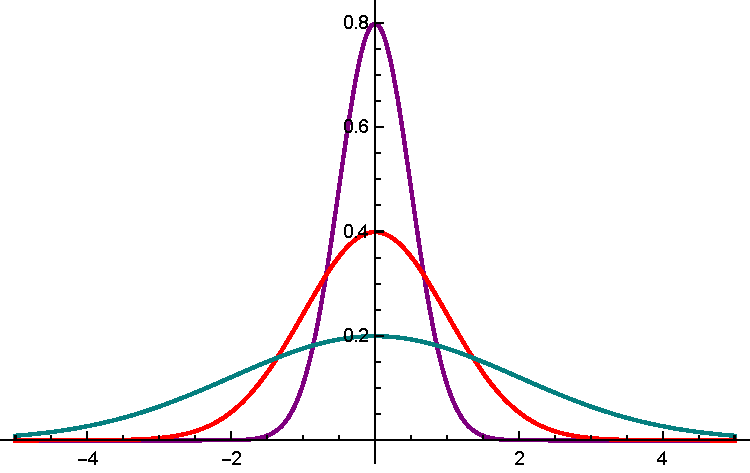
\includegraphics[scale=0.8]{body/image/NormalDistribution.pdf}
        \caption{不同方差下正态分布的概率密度曲线}
        \label{fig:NormalDistribution}
    \end{figure}

    $n$维正态随机变量$\bm x=(x_1,x_2,\cdots,x_n)^T$的概率密度函数为
    \begin{equation}\label{eq:NoramlDistribution}
        f_{\bm X}(\bm x)=\frac{1}{(2\pi)^{\frac{n}{2}}\abs{\bm C}^\frac{1}{2}}e^{-\frac{1}{2}(\bm x - \bm a)^T\bm C^{-1}(\bm x - \bm a)}
    \end{equation}
    其中$\bm a=\mathscr{E}[\bm x]$是$\bm x$的期望。$\bm C=\mathscr{E}[\bm{xx}^T]-\bm{aa}^T$是随机变量$\bm x$协方差矩阵。

    比如对于二维情况$n=2$
    \begin{equation*}
        \bm x=\begin{pmatrix}x_1\\x_2\end{pmatrix},\hspace{1em}\bm a=\begin{pmatrix}a_1\\a_2\end{pmatrix}
    \end{equation*}
    \vspace{-2ex}
    \begin{equation*}
        \begin{split}
            &\phantom{=}\bm{xx}^T-\bm{aa}^T\\
            &=\begin{pmatrix}
                x_1^2-a_1^2&x_1x_2-a_1a_2\\x_2x_1-a_2a_1&x_2^2-a_2^2
            \end{pmatrix}
        \end{split}
    \end{equation*}
    求期望得
    \begin{equation}
        \begin{split}
            \bm C   &=\mathscr{E}[\bm{xx}^T]-\bm{aa}^T\\
                    &=\begin{pmatrix}
                        \sigma_1^2&\rho\sigma_1\sigma_2\\
                        \rho\sigma_1\sigma_2&\sigma_2^2
                    \end{pmatrix}
        \end{split}
    \end{equation}
    带入到\eqaref{eq:NoramlDistribution}得
    \begin{equation}
        \begin{split}
            f_2(x_1,x_2)    &=\frac{1}{2\pi \sigma_1\sigma_2\sqrt{1-\rho^2}}\text{exp}\left\{-\frac{1}{2(1-\rho^2)}\right[\frac{(x_1-a_1)^2}{\sigma_1^2}\\
                            &\phantom{=}-2\rho\frac{(x_1-a_1)(x_2-a_2)}{\sigma_1\sigma_2}+\frac{(x_2-a_2^2)^2}{\sigma_2^2}\bigg]\bigg\}
        \end{split}
    \end{equation}
    取$a_1=a_2=0$,$\sigma_1=1$,$\sigma_2=1.5$,$\rho=0.4$,得概率密度函数如\figref{fig:2DNormalDistribution}。
    
    \begin{figure}[H]
        \centering
        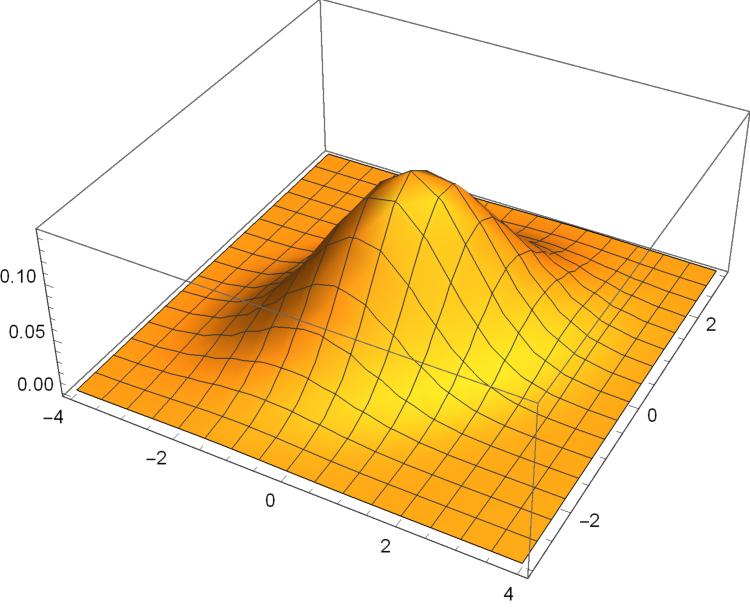
\includegraphics[scale=0.8]{body/image/2DNormalDistribution.pdf}
        \caption{二维正态分布概率密度曲面}
        \label{fig:2DNormalDistribution}
    \end{figure}

    因为正态分布可以由其一阶和二阶统计值(期望和方差)唯一确定,所以对于高斯过程,若为宽平稳过程,则也是严平稳过程。

    不难发现,协方差矩阵$\bm C$是一个对称矩阵,其特征根全为实数,可以对角化,即存在正交矩阵$\bm Q$和对角矩阵$\bm \Lambda$有
    \begin{equation}
        \bm C=\bm Q^T\bm\Lambda \bm Q
    \end{equation}
    那么\eqaref{eq:NoramlDistribution}可以重写为
    \begin{equation}
        f_{\bm X}(\bm x)=\frac{1}{(2\pi)^{\frac{n}{2}}\abs{\bm \Lambda}^\frac{1}{2}}e^{-\frac{1}{2}\bm y^T\bm \Lambda^{-1}\bm y},\hspace{1em}\bm y=\bm Q(\bm x - \bm a)
    \end{equation}
    可见$\bm x$可以表示成$n$个不相关的正态分布$\bm y$的线性组合,即$\bm x=\bm Q^T\bm y+\bm a$。

    而且不难知道,对于高斯分布,不相关与独立是相互等价的,即
    对于对角矩阵$\bm C=\text{diag}(\sigma_1^2,\sigma_2^2,\cdots,\sigma_n^2)$
    \begin{equation}
        \begin{split}
            f_{\bm X}(\bm x)    &=\frac{1}{(2\pi)^{\frac{n}{2}}\abs{\bm C}^\frac{1}{2}}e^{-\frac{1}{2}(\bm x - \bm a)^T\bm C^{-1}(\bm x - \bm a)}\\
                                &=\frac{1}{(2\pi)^{\frac{n}{2}}\displaystyle\prod_{i=1}^{n}\sigma_i}\text{exp}\left[-\frac{1}{2}\sum_{j=1}^{n}\frac{(x_i-a_i)^2}{\sigma_i^2}\right]\\
                                &=\prod_{i=1}^{n}\frac{1}{(2\pi)^{\frac{n}{2}}\sigma_i}\text{exp}\left[-\frac{1}{2}\frac{(x_i-a_i)^2}{\sigma_i^2}\right]\\
                                &=\prod_{i=1}^{n}f(x_i)
        \end{split}
    \end{equation}

    高斯分布常用相关函数如下:
    \paragraph{标准正态分布}
    \begin{equation}
        f(x)=\frac{1}{\sqrt{2\pi}}e^{-\frac{x^2}{2}}
    \end{equation}
    \paragraph{概率积分函数}
    \begin{equation}
        \Phi(x)=\frac{1}{\sqrt{2\pi}}\int_{-\infty}^{x}e^{-\frac{z^2}{2}}\dif z
    \end{equation}
    \paragraph{概率分布函数}
    \begin{equation}
        F(x)=\int_{-\infty}^{x}\frac{1}{\sqrt{2\pi}\sigma}e^{-\frac{(z-a)^2}{2\sigma^2}}\dif z=\Phi\left(\frac{x-a}{\sigma}\right)
    \end{equation}
    \paragraph{$Q$函数}
    \begin{equation}
        Q(x)=\frac{1}{\sqrt{2\pi}}\int_{x}^{\infty}e^{-\frac{z^2}{2}}\dif z=1-\Phi(x)
    \end{equation}
    \paragraph{误差函数}
    \begin{equation}
        \text{erf}(x)=\frac{1}{\sqrt{\pi}}\int_{-x}^{x}e^{-z^2}\dif z=2\Phi\left(\sqrt{2}x\right)-1
    \end{equation}

    \subsubsection{联合高斯}
    设$\bm Z=(Z_1,Z_2,\cdots,Z_n)^T$是一个随机列向量,其中$Z_1,Z_2,\cdots,Z_n$是独立同分布的标准正态随机变量,
    那么这$n$个随机变量和常数的线性组合$\bm X$服从联合分布,即
    \begin{equation}
        \bm X=\bm{AZ}+\bm b
    \end{equation}
    这一点通过之前的对角化也可以体现出来。

    \subsubsection{高斯过程}
    随机过程$X(t)$在$t_1,t_2,\cdots,t_n$时刻采样得到$n$个随机变量$X(t_1),X(t_2),\cdots,X(t_n)$,
    若对于任意的$n$和任意$t_1,t_2,\cdots,t_n$,$X(t_1),X(t_2),\cdots,X(t_n)$服从联合高斯分布,
    则称其为\emph{高斯过程}

    而且不难知道,高斯过程与确定信号的\emph{乘积}、\emph{卷积}之后的结果都是高斯过程。
    
\subsection{高斯白噪声}
    \subsubsection{定义}
    加性高斯白噪声(Additive White Gaussian Noise,AWGN)
    
    \paragraph{加}代表噪声是以线性的加法叠加在信号上,与之相对的是乘性。

    \paragraph{高斯}零均值高斯随机过程,而且高斯随机过程是所有结果中最坏的,以其作为模型可以估算出下界。

    \paragraph{白}借用光学中白的概念,白光是所有波长均匀混合在一起的结果,白噪声代表着各频率上的功率均匀相等。

    $n(t)$为高斯白噪声,其功率谱密度为
    \begin{equation}
        p_n(f)=\frac{N_0}{2},\hspace{1em}-\infty<f<\infty
    \end{equation}
    
    由\thmref{thm:Wiener_Khinchin}维纳--辛钦定理得
    \begin{equation}
        R_n(\tau)=\frac{N_0}{2}\delta(\tau)
    \end{equation}
    
    可见其功率无限大,对于任意两个不同时刻,这两个时刻的取值均不相关,
    因为为高斯过程,不相关即等价于独立。

    如果把高斯白噪声通过某个单位冲激响应为$h(t)$的线性时不变系统,输出$n(t)$,则得到
    \begin{align}
        P_n(f)&=\frac{N_0}{2}\abs{H(f)}^2\\
        \mathscr{E}[n^2(t)]&=\int_{-\infty}^{\infty}P_n(f)\dif f=\frac{N_0}{2}E_h
    \end{align}

    类似的,如果通过带宽为$B$,增益为1的理想低通滤波器,输出也是零均值平稳高斯过程功率是$N_0B$

    \subsubsection{加性高斯白噪声与确定信号的内积}
    对于通过高斯白噪声与确定信号$\varphi(t)$内积(也是一种求相关,或者说“投影”)确定的随机变量$X=\displaystyle\int_{-\infty}^{\infty}\varphi(t)n(t)\dif t$,
    其仍是期望为0的高斯随机变量,方差为$\dfrac{N_0}{2}E_\varphi$
    
    \Proof
    \begin{equation*}
        \begin{split}
            \mathscr{E}[X] &=\mathscr{E}\left[\int_{-\infty}^{\infty}\varphi(t)n(t)\dif t\right]=\int_{-\infty}^{\infty}\varphi(t)\mathscr{E}[n(t)]\dif t=0\\
            \mathscr{D}[X] &=\mathscr{E}\left[\int_{-\infty}^{\infty}\varphi(t_1)n(t_1)\dif t_1\int_{-\infty}^{\infty}\varphi(t_2)n(t_2)\dif t_2\right]\\
                           &=\mathscr{E}\left[\int_{-\infty}^{\infty}\int_{-\infty}^{\infty}n(t_1)n(t_2)\varphi(t_1)\varphi(t_2)\dif t_\dif t_2\right]\\
                           &=\int_{-\infty}^{\infty}\int_{-\infty}^{\infty}\mathscr{E}[n(t_1)n(t_2)]\varphi(t_1)\varphi(t_2)\dif t_1\dif t_2\\
                           &=\int_{-\infty}^{\infty}\int_{-\infty}^{\infty}\frac{N_0}{2}\delta(t_1-t_2)\varphi(t_1)\varphi(t_2)\dif t_1\dif t_2\\
                           &=\frac{N_0}{2}\int_{-\infty}^{\infty}\varphi^2(t)\dif t\\
                           &=\frac{N_0}{2}E_\varphi
        \end{split}
    \end{equation*}

    进而,如果高斯白噪声$n(t)$和两个信号$\varphi_1(t)$、$\varphi_2(t)$分别做内积(投影)得到两个服从高斯分布的随机变量$Z_1$、$Z_2$,
    类似上面的过程,可以得到二者的相关性
    \begin{equation}
        \mathscr{E}[Z_1Z_2]=\frac{N_0}{2}\int_{-\infty}^{\infty}\varphi_1(t)\varphi_2(t)\dif t
    \end{equation}
    可见如$\varphi_1(t)$、$\varphi_2(t)$正交,$Z_1$、$Z_2$不相关,等价于独立。

    同时,如果$\varphi_1(t)$、$\varphi_2(t)$是两个不同频带的带通滤波器的单位冲激响应,
    由\eqaref{eq:inner}得,
    \begin{equation}
        \int_{-\infty}^{\infty}\varphi_1(t)\varphi_2(t)\dif t=\int_{-\infty}^{\infty}\Phi_1(f)\Phi_2^*(f)\dif f
    \end{equation}
    可见,在两个不同子频带上的高斯白噪声得的分量相互独立。

    进而推广,$n$个两两正交的归一化正交函数$\varphi_1(t),\varphi_2(t),\cdots,\varphi_n(t)$上,
    $n(t)$投影均为$Z_i\sim\mathscr{N}(0,\dfrac{N_0}{2})$,是服从同一分布且两两独立的正态分布。

    对于低通限带高斯白噪声,其功率谱密度为
    \begin{equation}
        P_n(f)=\frac{N_0}{2}\text{rect}\left(\frac{f}{2f_H}\right)
    \end{equation}
    其自相关函数为n
    \begin{equation}
        R_n(\tau)=\frac{N_0}{2}2f_H\text{sinc}(2f_H\tau)=\sigma_n^2\text{sinc}(2f_H\tau)
    \end{equation}

    可见
    \begin{equation}
        R_n\left(\frac{k}{2f_H}\right),\hspace{1em}k=\pm 1,\pm 2,\pm 3,\cdots
    \end{equation}
    故应该以$\dfrac{1}{2f_H}$的整数倍时间间隔抽样,才能获得无关(等价于独立)的样本。

    \subsubsection{窄带平稳高斯过程}
    
    结合之前的内容,不难做出一下\emph{}{结论}:
    均值为 0 的窄带高斯\Emph{平稳}过程 $X(t)$
    \paragraph{}其同相分量$X_c(t)$和正交分量$X_s(t)$也是高斯平稳随机过程。
    \paragraph{}同相分量与正交分量均值为 0 且方差等于$X(t)$的方差。
    \paragraph{}在同一时刻,$X_c(t)$和$X_s(t)$相互独立。
    \paragraph{}\emph{如果$P_X(f)$关于$f_c$对称,则$X_c(t)$和$X_s(t)$是独立的随机过程。}
    \vspace{2ex}

    不难证明的是,限带平稳高斯过程的复包络$A(t)e^{j\varphi{t}}=n_c(t)+jn_s(t)$,其模值$A$服从瑞利分布
    \begin{equation}
        p_A(a)=\frac{a}{\sigma^2}e^{-\frac{a^2}{2\sigma^2}}
    \end{equation}
    其相位在区间$[0,2\pi)$上服从均匀分布。

    如果对上述信号上叠加一个余弦波$A\cos(2\pi f_ct)$后,复包络为$X_L(t)=[A+n_c(t)]+jn_s(t)$,
    其包络(模值)$R(t)=\abs{X_L(t)}$服从莱斯分布
    \begin{equation}
        p_R(r)=\frac{r}{\sigma^2}e^{-\frac{r^2+A^2}{2\sigma^2}}I_0\left(\frac{Ar}{\sigma^2}\right)
    \end{equation}

\subsection{匹配滤波器}
    匹配滤波器,即\emph{某一特定时刻的输出信噪比最大的线性滤波器}。
    
    一单位冲激响应为$h(t)$的系统,输入为$x(t)=s(t)+n(t)$,输出为$y(t)=s_0(t)+n_0(t)$。
    输出信号的瞬时功率为$\abs{s(t)}^2$,输出噪声的统计平均功率为$\mathscr{E}\left[\abs{n_0(t)}^2\right]$。
    其中
    \begin{align}
        s_0(t)&=\mathscr{F}^{-1}[H(f)S(f)]=\int_{-\infty}^{\infty}H(f)S(f)e^{j2\pi ft}\dif f\\
        \mathscr{E}\left[\abs{n_0(t)}^2\right]&=\frac{N_0}{2}\int_{-\infty}^{\infty}\abs{H(f)}^2\dif f=\frac{N_0}{2}E_h
    \end{align}

    那么在输出时刻$t_0$的瞬时信噪比为:
    \begin{equation}
        r_0=\frac{\abs{s(t)}^2}{\mathscr{E}\left[\abs{n_0(t)}^2\right]}=\frac{\abs{\displaystyle\int_{-\infty}^{\infty}H(f)S(f)e^{j2\pi ft_0}\dif f}^2}{\dfrac{N_0}{2}\displaystyle\int_{-\infty}^{\infty}\abs{H(f)}^2\dif f}
    \end{equation}
    由柯西施瓦茨不等式\footnote{Cauchy--Schwarz不等式有很多种形式,这里采用的是\begin{equation*}
        \abs{\int_{-\infty}^{\infty}X(f)Y^*(f)\dif f}^2\leq \left[\int_{-\infty}^{\infty}\abs{X(t)}^2\dif f\right]\cdot\left[\int_{-\infty}^{\infty}\abs{Y(t)}^2\dif f\right]
    \end{equation*}
    $Y(f)=K\cdot X(t)$时取到等号,其中$K\in\mathbb{C}$}
    得
    \begin{equation}
        \begin{split}
            r_0=\frac{\abs{\displaystyle\int_{-\infty}^{\infty}H(f)S(f)e^{j2\pi ft_0}\dif f}^2}{\dfrac{N_0}{2}\displaystyle\int_{-\infty}^{\infty}\abs{H(f)}^2\dif f}&\leq\frac{\left[\displaystyle\int_{-\infty}^{\infty}\abs{H(t)}^2\dif f\right]\cdot\left[\displaystyle\int_{-\infty}^{\infty}\abs{S(t)}^2\dif f\right]}{\dfrac{N_0}{2}\displaystyle\int_{-\infty}^{\infty}\abs{H(f)}^2\dif f}\\
            &=\frac{2\displaystyle\int_{-\infty}^{\infty}\abs{S(f)}^2\dif f}{N_0}\\
            &=\frac{2E_s}{N_0}
        \end{split}
    \end{equation}

    可见最大信噪比与输入信号其他性质无关,仅与信号本身得能量有关。
    为了使$r_0$取到最大值$\dfrac{2E_s}{N_0}$,需满足
    \begin{equation}
        H(f)=K\cdot S^*(f)e^{-j2\pi ft_0}
    \end{equation}
    做反变换得
    \begin{equation}
        h(t)=K\cdot s(t_0-t)
    \end{equation}
    相当于原信号波形的镜像平移,考虑到滤波器的因果性(物理可实现性),一般取$t_0$为时间有限的信号$s(t)$消失的时间$T$。
    
    实际上匹配滤波器相当于一个相关器
    \begin{equation}
        \begin{split}
            y(t)&=s(t)*h(t)\\
                &=\int_{-\infty}^{\infty}s(t-\tau)h(\tau)\dif \tau\\
                &=K\cdot\int_{-\infty}^{\infty}s(t-\tau)s(T-\tau)\dif \tau
        \end{split}
    \end{equation}
    考虑输入的信号为实信号,对比\eqaref{eq:RX}
    \begin{equation}
        y(t)=K\cdot R_s(t-T)
    \end{equation}
    同样不难知,在$t-T=0$取最大值$K\cdot R_s(0)=K\cdot E_s$


    

